\documentclass[]{article}
\usepackage{amsmath}
\usepackage{graphicx}
\usepackage[margin = 2cm]{geometry}
\usepackage{tcolorbox}
\usepackage{cite}
\usepackage{booktabs}
\usepackage{siunitx}
\usepackage{subcaption}
\usepackage{amssymb}
\bibliographystyle{unsrt}
\usepackage{hyperref}
%\pagestyle{headings}

\usepackage{fancyhdr}
\pagestyle{fancy}

%\fancyhf{}
%\rhead{Overleaf}
%\lhead{Guides and tutorials}
%\rfoot{Page \thepage}



\begin{document}


\section{Move to $\ell b$ classifier}
\footnotetext{Date: Early August 2020}
\subsection{Motivation}
Move due to poor performance on event level BDT (was using 50\% TRF and 50\% testing/training). ST, minMax, HT and a few other variables performed better than the BDT $\rightarrow$ most likely due to the fact that the BDT score variable had half the MC than just taking the full MC dataset as normal.
\subsection{Different Iterations/Setups}
Common setup:
\begin{itemize}
	\item use $t\bar{t}$ Bakoven sample (Ntuple-level selection of 1 lepton)
	\item Signal: $\ell b$ from the same top
	\item Signal: $\ell b$ \textbf{NOT} from the same top
\end{itemize}
\subsubsection{Matching $\ell$ \textbf{AND} $b$ to truth}

Match $\ell$ and $b$ to their truth particles, by use of smallest $\Delta R$. Small $\Delta R$ is indication of a good match to truth. 


\begin{itemize}
	\item Signal: $\ell$ and $b$ with the smallest $\Delta R$ (below some threshold $\rightarrow$ 0.3) and come from the same top
	\item Background: $\ell$ and $b$ with the smallest $\Delta R$ (below some threshold $\rightarrow$ 0.3) and DON'T come from the same top
	
\end{itemize}
\fbox{
Note: threshold chosen of 0.3 is VERY loose}
\begin{figure}[!h]
	\centering
	\captionsetup[subfigure]{labelformat=empty}
	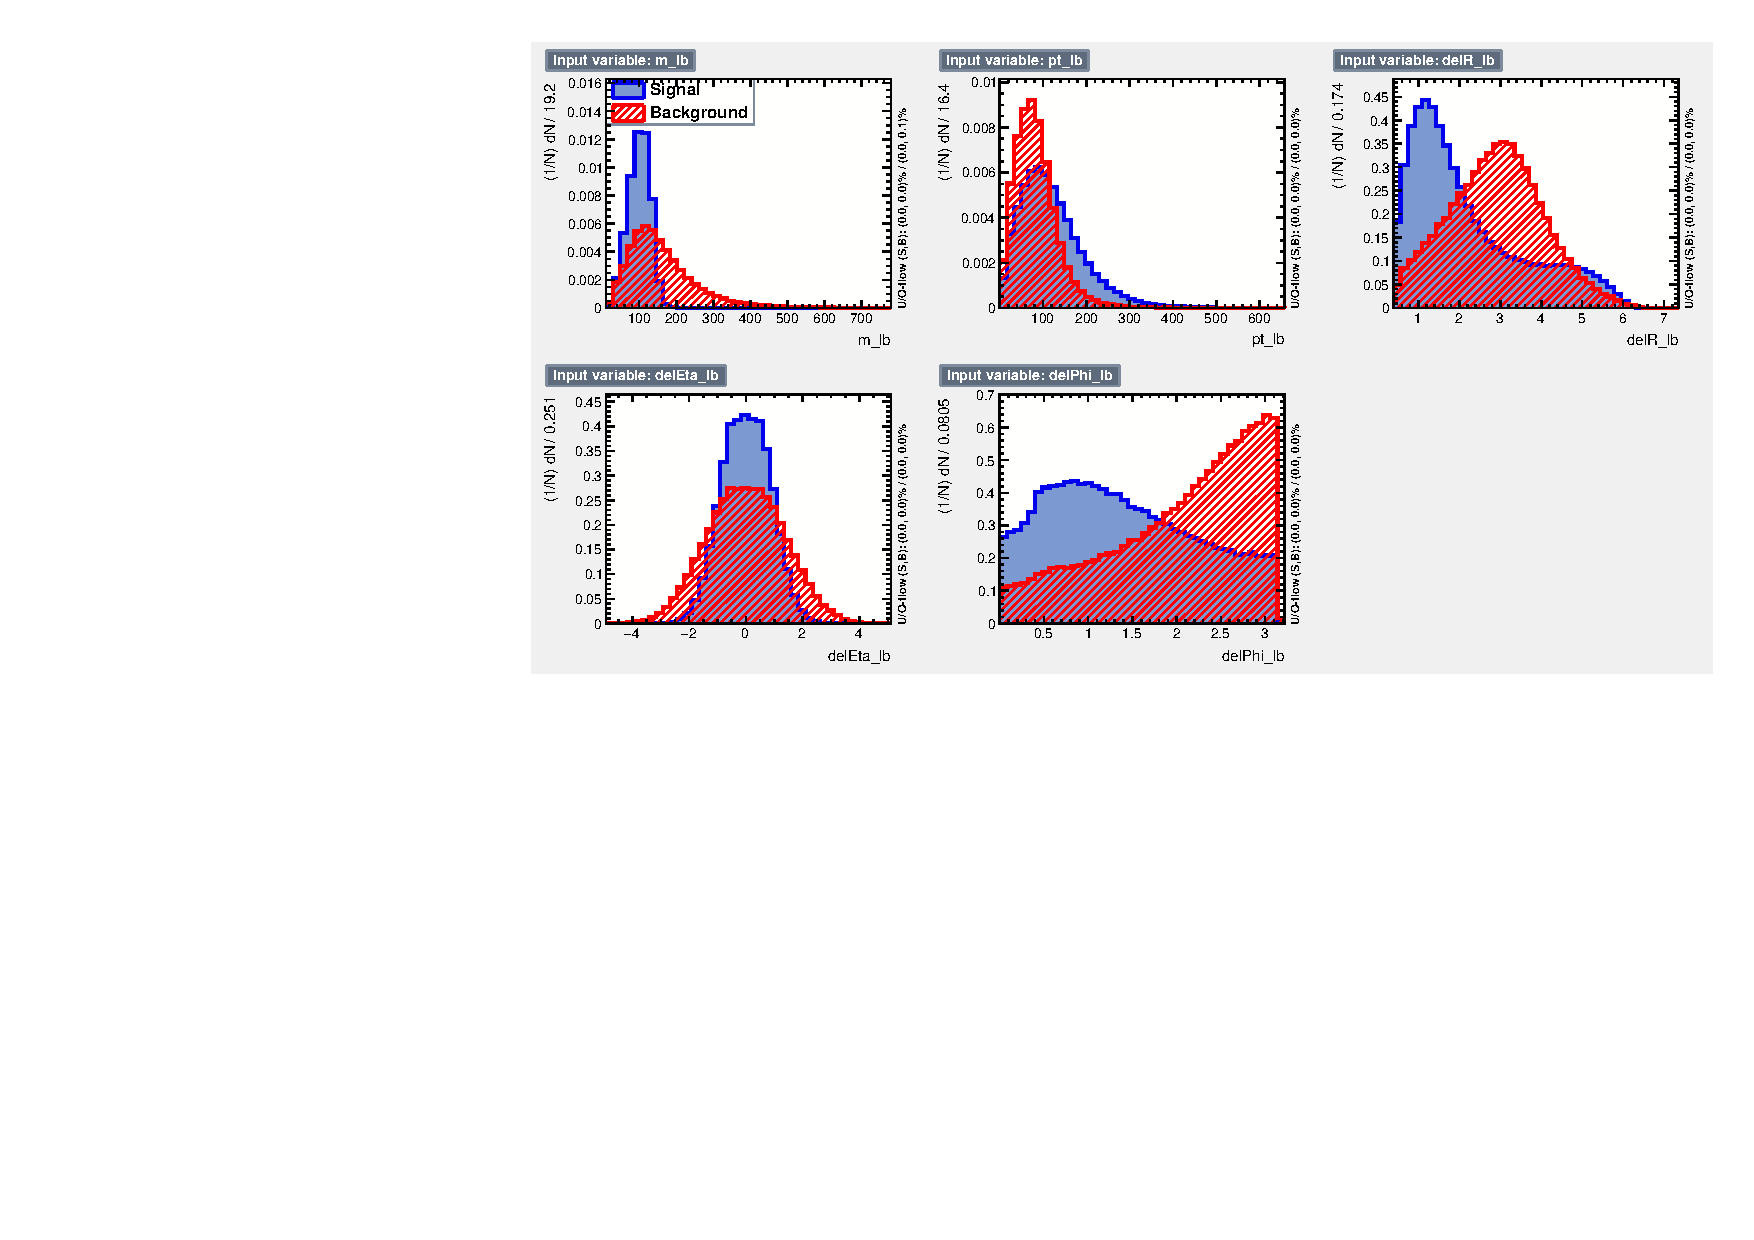
\includegraphics[width=0.7\textwidth]{variables.pdf}
	\caption{Input variables}
\end{figure}

\begin{itemize}
	\item Num events\footnote{James says this is sufficient and any more would just slow down training} training $\sim$ 240 000 (sig and back)
	\item Num events testing $\sim$ 60 000 (sig and back)
\end{itemize}
$\star$ Check non-linear correlation coefficient graphs (In TMVAGui)
\pagebreak

\begin{figure}[!h]
	\begin{subfigure}[b]{0.4\textwidth}
		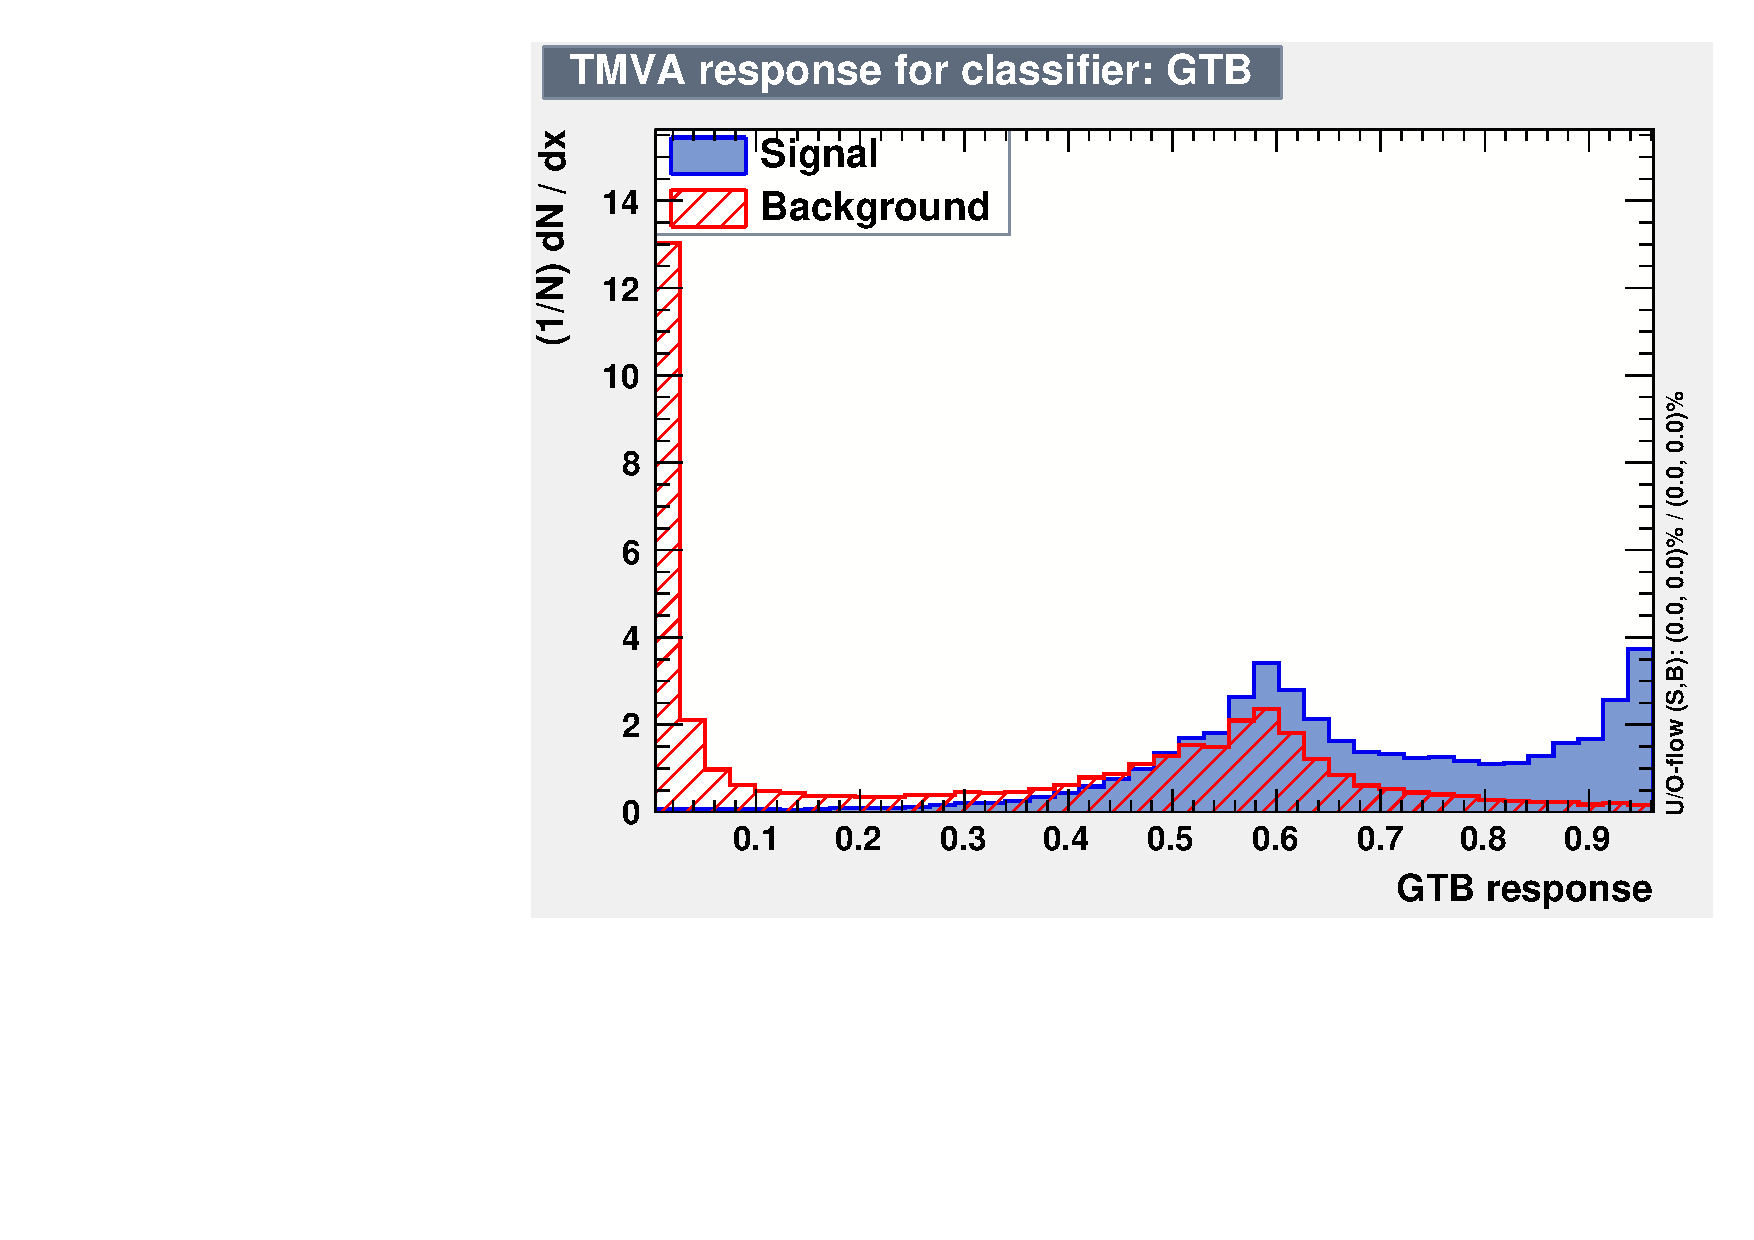
\includegraphics[width=\textwidth]{gtb_response.pdf}
		
	\end{subfigure}
	%
	\begin{subfigure}[b]{0.4\textwidth}
		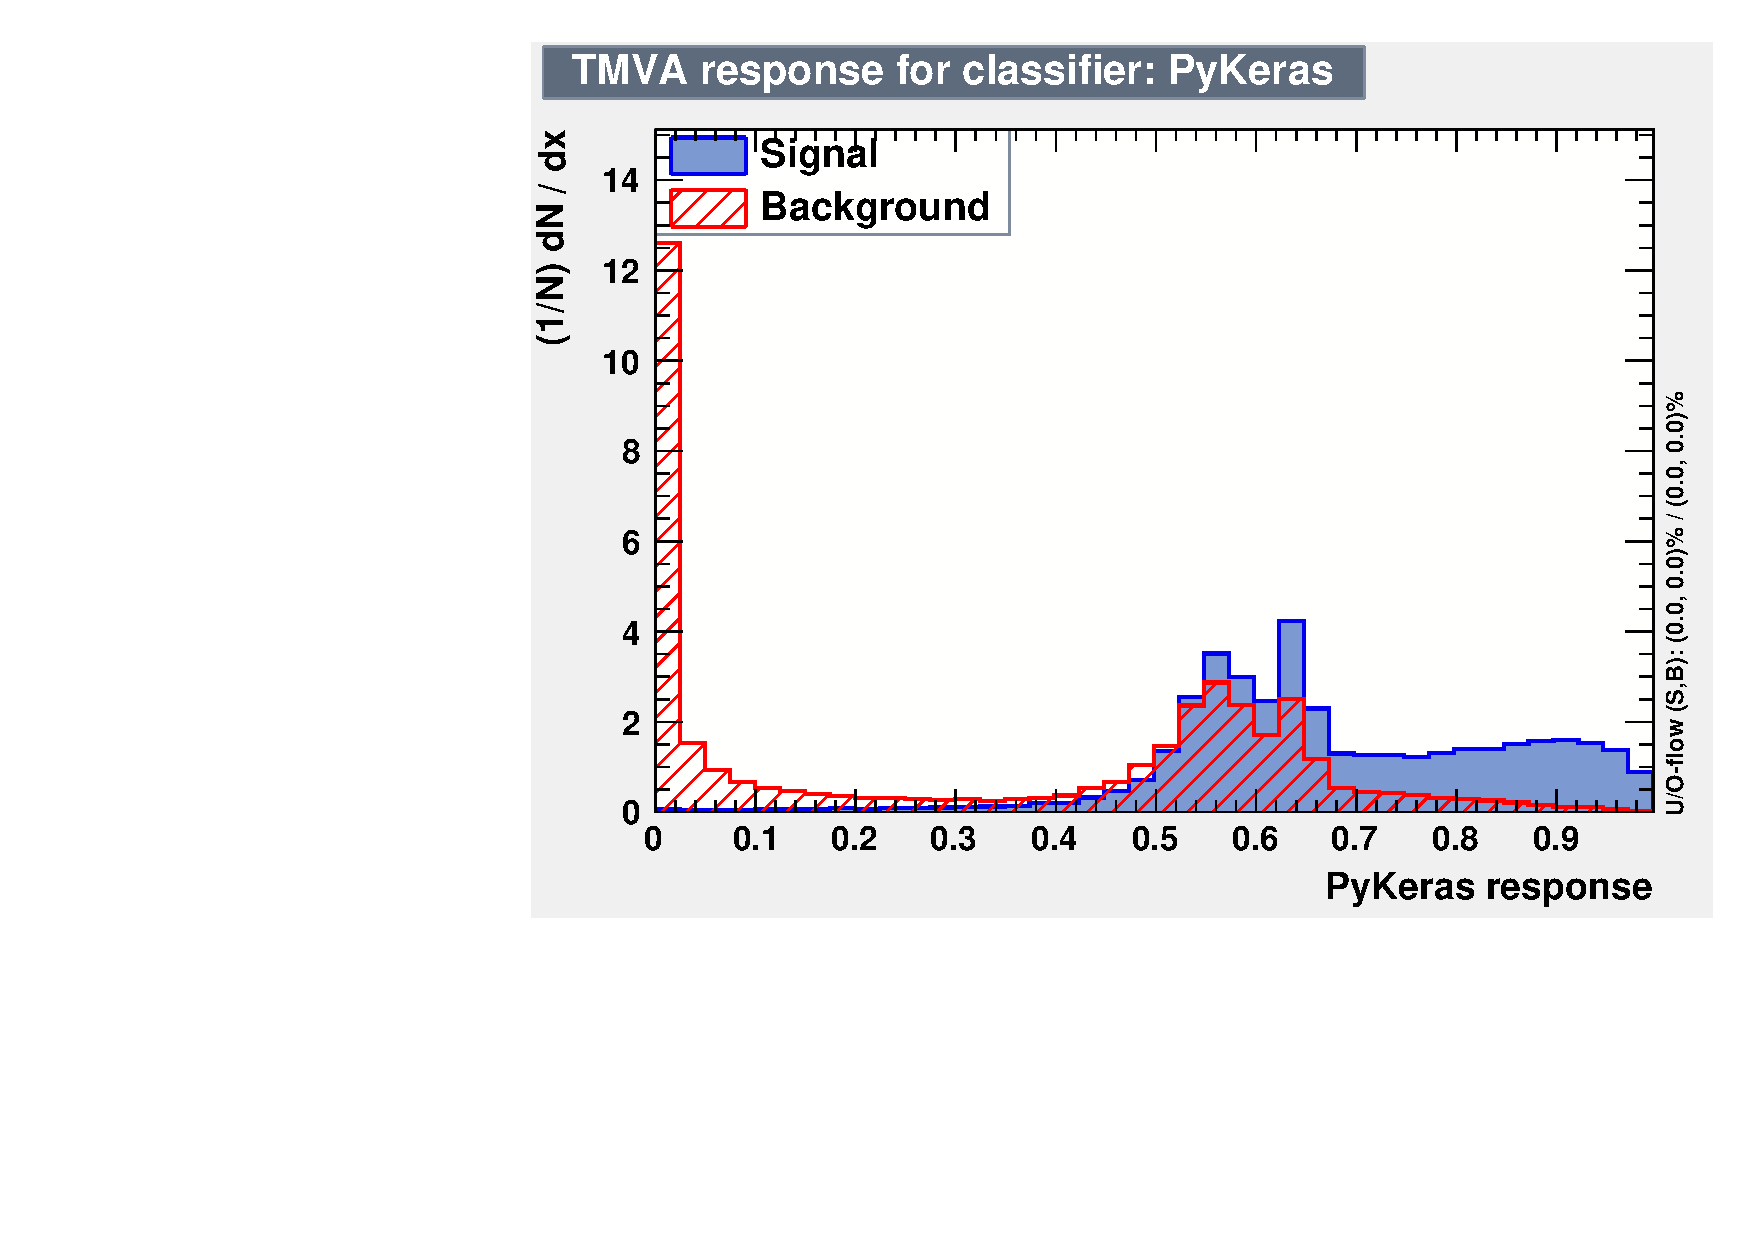
\includegraphics[width=\textwidth]{keras_response.pdf}
		
	\end{subfigure}
\end{figure}
$\star$ Weird bump?\\ \\
\underline{\large Results:}
\begin{figure}[!h]
	\begin{subfigure}[b]{0.4\textwidth}
		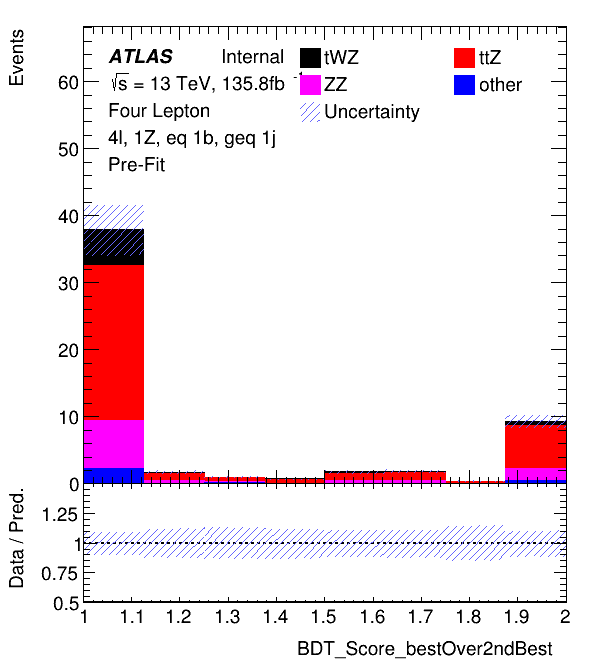
\includegraphics[width=\textwidth]{bdt_res_1.png}
		
	\end{subfigure}
	%
	\begin{subfigure}[b]{0.4\textwidth}
		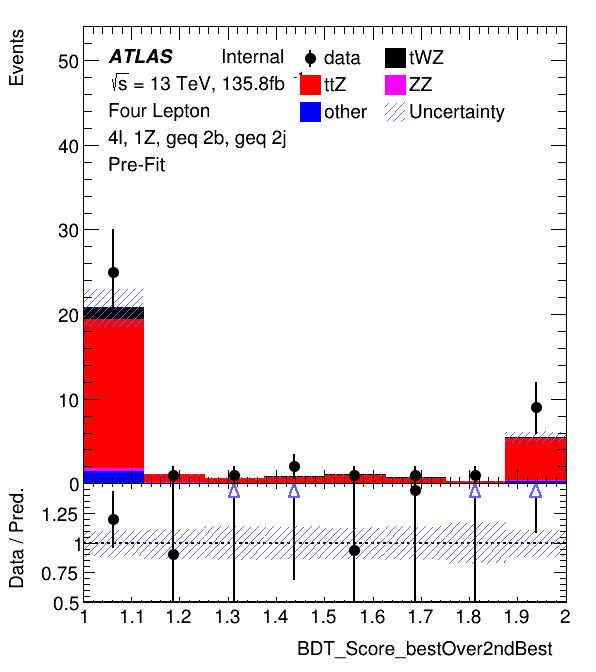
\includegraphics[width=\textwidth]{bdt_res_2.png}
		
	\end{subfigure}
\end{figure}
\\\\
\fbox{Limit $\rightarrow$ \textcolor{blue}{2.429} (All ASIMOV), \textcolor{red}{2.488} (Data in CR)}\\\\
Previously (Full Run 2 $m(\ell b)_{minMax}$) $\rightarrow$ \textcolor{blue}{2.474} (All ASIMOV), \textcolor{red}{2.535} (Data in CR)
\\\\
\fbox{** Figured out that the '-1' default value is being used in the fit (underflow), as can see in first bin **}

\subsubsection{Matching $\ell b$ system to truth}



\section{Delft Ntuples}
\subsection{Yield Discrepancy}
\fbox{Supposed difference between Delft and Constantia which has the largest effect $\rightarrow$ using a tighter lepton isolation parameter} \\\\
This causes much less stats/yields in Delft (compared to Constantia) $\rightarrow$ also seen in Cameron's analysis. I compared 2018 Constantia and Delft 2018 ($ttZ$ region), 1 data event in Constantia and 0 in Delft. This was concerning, so looked at INT note to see stats/yields Full Run 2 Constantia had. INT note had around 40 data events (would expect 2018 Constantia to have more than 1, probably around 16 (since luminosity of mc16e is a bit less than half of Full Run 2 luminosity)). The only differences between INT note plot and 2018 Constantia control plot are that we are using Full Run 2 and the 77$\%$ btag WP (referring to INT note plots).\\\\
Recall:
\begin{itemize}
	\item[-] Tight jet: 77 WP or less
	\item[-] Loose jet: 85 WP
\end{itemize}


\begin{itemize}
	\item Delft 2018: 0 $ttZ$ data events ($\geq$ 1 tight, $\geq$ 1 loose, loose $+$ tight $=$ 2)
	\item Constantia 2018: 1 $ttZ$ data event ($\geq$ 1 tight, $\geq$ 1 loose, loose $+$ tight $=$ 2)
	\item Constantia in INT Note (Full Run 2): $\sim ttZ$ 40 data events ($\geq$ 1 tight, $\geq$ 0 loose, loose $+$ tight $=$ 2)
\end{itemize}

Changed Constantia 2018 $ttZ$ region to $\geq$ 1 tight, $\geq$ 0 loose, loose $+$ tight $=$ 2 (essentially what is in INT note (these plots are before this bjet WP was implemented)). This gave us the expected total number of events, $\approx$ 17.








\end{document}
